\documentclass[a4paper, 12pt, oneside]{report}

\newcommand{\plogo}{\fbox{$\mathcal{PL}$}} 
\usepackage{geometry}
\geometry{margin=1in}
\usepackage{graphicx}
\usepackage{graphics}
\usepackage{float}
\usepackage{booktabs}
\usepackage{caption}
\usepackage{longtable}
\usepackage{array}
\usepackage{enumitem}
\usepackage{fancyhdr}
\usepackage{titlesec}
\usepackage{microtype}
\usepackage{listings}
\usepackage[table,xcdraw]{xcolor}
\usepackage[utf8]{inputenc} 
\usepackage[T1]{fontenc} 
\usepackage{fouriernc} 
\usepackage{subcaption}
\usepackage{tikz}
\usepackage{pgfplots}
\usepackage{graphics}
\usepackage{longtable}
\usepackage[nottoc]{tocbibind}
\usepackage{url}
\usepackage{hyperref}
\usepackage{amsmath}
\usepackage{lipsum}

\hypersetup{
	colorlinks=true,
	linkcolor=blue,
	urlcolor=blue,
	citecolor=blue
}

% Headers/footers and section styling (research-paper feel)
\pagestyle{fancy}
\fancyhf{}
\fancyhead[LE,RO]{DevForge Project Report}
\fancyhead[RE,LO]{\leftmark}
\fancyfoot[CE,CO]{\thepage}
\setcounter{secnumdepth}{3}
\setcounter{tocdepth}{3}
	itlespacing*{\section}{0pt}{*3}{*1}
	itlespacing*{\subsection}{0pt}{*2}{*0.8}
	itlespacing*{\subsubsection}{0pt}{*1.5}{*0.6}
\microtypecontext{spacing=nonfrench}
\lstset{basicstyle=\ttfamily\small,breaklines=true,frame=single}

\begin{document}
\begin{titlepage}
\centering
\vspace*{\baselineskip}
\vspace{0.75\baselineskip}
{\LARGE DevForge: Web-Based IDE with Persistent Docker Containers}
\vspace{0.75\baselineskip}
\vspace{2\baselineskip}
{A project report submitted in partial fulfillment of the requirements of the degree}
\\[0.25\baselineskip]
{of Bachelor of Technology}
\\[1.0\baselineskip]
{in Computer Science and Engineering}
\vspace*{5\baselineskip}
\begin{tabular}{p{0.45\textwidth} p{0.45\textwidth}}
	extbf{Submitted by:} & \textbf{Supervised by:} \\
Your Name & Supervisor Name \\
Roll No: XXXXXXX & Department/Institute \\
\end{tabular}
\vfill
\begin{center}
\includegraphics[width=5cm]{report_file/iiit manipur.png}
\end{center}
{\scshape\small Department of Computer Science and Engineering\\ Indian Institute of Information Technology Senapati, Manipur \\ \today}
\end{titlepage}
	
	\begin{center}
	{ \LARGE \textbf{Declaration}}
	\end{center}
	I hereby declare that the work presented in this report titled \textbf{\emph{DevForge: Web-Based IDE with Persistent Docker Containers}} is an authentic record of my own work carried out during the academic term. All sources of information have been duly acknowledged through proper citations and references.
	\\[1cm]
	\hfill Signature: \rule{4cm}{0.4pt}
	\\[0.4cm]
	\hfill Name: \rule{5cm}{0.4pt}
	\\[0.4cm]
	\hfill Roll No: \rule{4cm}{0.4pt}
	\\[0.8cm]
	Date: \rule{4cm}{0.4pt}

	\newpage

	\begin{center}
		hispagestyle{empty}
	\begin{table}
	\centering
	\includegraphics[scale=0.2]{report_file/iiit manipur.png}
	\begin{tabular}{l}
	Department of Computer Science and Engineering \\
	Indian Institute of Information Technology Senapati, Manipur \\
	\end{tabular}
	\end{table}
	\par\noindent\rule{\textwidth}{0.4pt}
		extbf{Supervisor Certificate}\\[1.0cm]
	\linespread{1.13}
	\large{This is to certify that the project report entitled \textbf{\emph{DevForge: Web-Based IDE with Persistent Docker Containers}} is a bona fide record of work carried out by the student under my supervision.}\\[2.0cm]
	\hspace*{2.6in}\large{Signature of Supervisor}\\[0.3cm]
	\hspace*{2.5in}\textbf{(Name and Designation)}\\[0.5cm]
	\end{center}

	\newpage

	\begin{abstract}
	DevForge is a full-stack, web-based integrated development environment (IDE) that provisions persistent Docker containers per project and provides a modern editing experience in the browser using the Monaco editor. The platform is built with Next.js 14 (App Router) and TypeScript, and integrates MongoDB for metadata, Redis for port allocation and caching, NextAuth for authentication, and Docker management via dockerode. Key features include multi-project management, file system operations, a real-time terminal view, and automatic port management for frontend and backend services. This report details the motivation, requirements, architecture, implementation, and evaluation of DevForge, and positions it relative to existing cloud IDE solutions such as GitHub Codespaces and Gitpod.\cite{codespaces,gitpod}
	\end{abstract}

	\begin{center}
	{ \LARGE \textbf{Acknowledgment}}
	\end{center}
	I would like to thank my supervisor for guidance and feedback throughout the project, and my peers for their helpful discussions and reviews. The open-source communities behind Next.js, Docker, MongoDB, Redis, and Monaco provided invaluable tooling and documentation.\cite{nextjs,docker,mongodb,redis,monaco}
	\\[0.6cm]
	\hfill \rule{5cm}{0.4pt}\\[-0.2cm]
	\hfill Signature
	I would like to express my gratitude to my supervisor, Prof. Motilal, for his invaluable guidance throughout the course of this project. His support and expertise made it possible to develop this simulation system successfully. I am also thankful to my peers and my family, whose encouragement and input helped shape the outcome of this project.
	
	\hspace{7cm} Sameer Badami

	\tableofcontents
	\chapter{Introduction}

\section{Overview of the Project}
The F1 Simulation Project is a comprehensive C-based program designed to simulate Formula 1 races. It provides users with the opportunity to select car manufacturers, drivers, venues, and specific race parameters, such as the number of laps. The project is structured to handle various input types, process race simulations based on complex car statistics, and generate accurate results in a user-friendly format. The primary goal of this project is to simulate an authentic racing experience, while also offering detailed performance analysis through lap time tracking and podium standings.

\section{Motivation and Problem Statement}
Motorsports enthusiasts and developers often seek ways to emulate real-world racing scenarios through simulations. This project aims to address this by providing a streamlined interface for race simulation, while also handling intricate race dynamics, such as car performance factors (horsepower, reliability, aerodynamics) and venue-specific conditions. The problem is to create a system that balances realism with simplicity, making it accessible to both casual users and those interested in a more analytical approach to racing data.

\section{Scope of the Project}
This project focuses on:
\begin{itemize}
    \item Designing a race simulation engine that factors in car performance statistics and venue attributes.
    \item Offering a customizable user interface where users can choose from various car manufacturers, drivers, and venues.
    \item Calculating race results, including lap times, podium standings, and race commentary.
    \item Providing detailed output that mimics real-life race analysis.
\end{itemize}

\section{Objectives}
The main objectives of the F1 Simulation Project are:
\begin{itemize}
    \item To develop a C-based program capable of simulating Formula 1 races.
    \item To calculate race results based on car performance, venue characteristics, and lap conditions.
    \item To present race outcomes in a user-friendly format, including podium standings and race commentary.
    \item To track driver statistics over multiple simulations and analyze performance trends.
\end{itemize}

\section{Structure of the Report}
The report is structured as follows:
\begin{itemize}
    \item Chapter 2 covers the Literature Survey, reviewing related work in motorsport simulations and F1 statistics tracking systems.
    \item Chapter 3 describes the Requirement Engineering phase, focusing on user requirements, functional requirements, and system specifications.
    \item Chapter 4 outlines the System Design, detailing the architecture, process flow, and input/output design of the project.
    \item Chapter 5 explains the Implementation, presenting the C code structure and highlighting key algorithms used in race simulation.
    \item Chapter 6 presents the Results, showcasing the race outcomes, statistics, and system performance.
    \item Chapter 7 concludes the report with an evaluation of the project and suggestions for future enhancements.
\end{itemize}

\newpage




	\chapter{Literature Survey}

\section{Introduction}
This chapter presents a comprehensive survey of existing literature and works related to motorsport simulation, Formula 1 racing analysis, and statistics tracking systems. The purpose of this literature survey is to understand current trends and identify key techniques used in simulating races and tracking driver performance. These insights inform the development of the F1 Simulation Project and ensure that the system we design aligns with industry standards.

\section{Review of Existing Race Simulations}
Various race simulation projects have been developed, ranging from academic prototypes to commercial games. Some notable examples include:
\begin{itemize}
    \item \textbf{Codemasters' F1 Series:} A widely recognized commercial game that simulates Formula 1 races with highly detailed graphics and realistic car physics. The game uses advanced algorithms to model real-world factors such as tire degradation, weather conditions, and driver behavior. However, the system is highly complex and requires significant computational resources.
    \item \textbf{Open Source Racing Simulation (OSRSim):} An open-source project that allows users to simulate races in various motorsport disciplines, including Formula 1. OSRSim provides a simplified user interface and focuses more on ease of use than on detailed race dynamics.
\end{itemize}

\section{Race Analysis and Driver Performance Tracking}
A key component of any race simulation system is the ability to track and analyze driver performance. In the professional racing world, this analysis is essential for both real-time race strategies and post-race reviews. Several existing systems offer insights into how this can be achieved:
\begin{itemize}
    \item \textbf{Race Logic's VBOX Motorsport:} A performance tracking system that uses GPS data to measure lap times, cornering speed, and braking points. This system is used by real-world teams to optimize car setup and driver performance.
    \item \textbf{Motec's Data Logging System:} An advanced system used in professional motorsport to collect detailed telemetry data during races. It helps engineers make data-driven decisions on car setup, driver performance, and race strategy.
\end{itemize}

\section{Challenges in Race Simulations}
Several challenges arise when developing race simulations, particularly when trying to balance realism with simplicity. These include:
\begin{itemize}
    \item \textbf{Realistic Car Physics:} Implementing accurate car physics requires complex algorithms to account for variables such as tire friction, downforce, and engine power. Simplifying these dynamics while maintaining a sense of realism is difficult.
    \item \textbf{Real-time Performance Analysis:} Tracking lap-by-lap performance in real-time, particularly over a network of multiple drivers, can be computationally intensive. The F1 Simulation Project will address this by focusing on a single-player mode, where calculations are made locally.
    \item \textbf{Dynamic Weather Conditions:} Weather plays a significant role in real-world racing, but simulating dynamic weather patterns adds a layer of complexity to race simulations. The F1 Simulation Project will exclude weather conditions to keep the scope manageable.
\end{itemize}

\section{Conclusion}
The literature review reveals that existing systems prioritize either realism (e.g., Codemasters' F1 series) or simplicity (e.g., OSRSim). The F1 Simulation Project aims to strike a balance between the two by offering a user-friendly interface while still incorporating key performance factors such as horsepower, aerodynamics, and reliability. Additionally, race performance will be tracked on a lap-by-lap basis, offering insights into driver performance without the overhead of complex telemetry systems.

\newpage

	\chapter{Requirement Engineering}

\section{Introduction}
Requirement engineering is a crucial phase in software development, where user needs are gathered, analyzed, and translated into functional and non-functional requirements. This chapter outlines the requirements for the F1 Simulation Project based on the user interactions, system functionality, and performance objectives. The goal is to ensure that the system aligns with user expectations and provides an intuitive, responsive race simulation experience.

\section{User Requirements}
The primary users of the F1 Simulation Project are motorsport enthusiasts who wish to simulate Formula 1 races, and the secondary users are evaluators who analyze the simulation results. The user requirements are as follows:
\begin{itemize}
    \item \textbf{Easy-to-use interface:} Users should be able to easily select cars, drivers, and venues without complicated navigation.
    \item \textbf{Customizable race parameters:} Users should be able to input performance values such as horsepower, reliability, and aerodynamics.
    \item \textbf{Detailed race results:} Users expect detailed output, including lap-by-lap statistics, podium standings, and race commentary.
    \item \textbf{Realistic performance calculations:} The system must calculate race results based on realistic factors such as horsepower and venue characteristics.
\end{itemize}

\section{Functional Requirements}
The functional requirements define the core functionality that the F1 Simulation Project must deliver:
\begin{itemize}
    \item \textbf{Race Simulation:} The system must simulate a Formula 1 race, considering user-selected parameters such as car manufacturer, driver, venue, and number of laps.
    \item \textbf{Statistics Tracker:} The system must track driver statistics, including lap times, race positions, and overall performance.
    \item \textbf{Podium Standings Display:} The system must calculate and display podium standings based on race outcomes.
    \item \textbf{Commentary Generator:} The system must generate race commentary based on the car manufacturer and driver performance.
    \item \textbf{Input Interface:} The system must provide a user-friendly interface where users can select options from dropdown menus for car manufacturers, drivers, and venues.
\end{itemize}

\section{Non-functional Requirements}
Non-functional requirements specify the performance and usability aspects of the system:
\begin{itemize}
    \item \textbf{Performance:} The system must calculate race results within a few seconds after input submission to maintain user engagement.
    \item \textbf{Scalability:} The system should be designed to handle additional features or user inputs in future versions.
    \item \textbf{Reliability:} The system should provide consistent, accurate results based on user input without errors or crashes.
    \item \textbf{Usability:} The user interface must be intuitive, with clear options for selecting drivers, cars, and venues.
\end{itemize}

\section{System Specifications}
The system specifications define the technical parameters under which the project will operate:
\begin{itemize}
    \item \textbf{Programming Language:} The F1 Simulation Project is implemented in C.
    \item \textbf{System Environment:} The system will be developed and tested on a Linux-based environment (Ubuntu) using the GCC compiler.
    \item \textbf{Hardware Requirements:} The system should run on a standard PC with at least 4GB RAM and 1GHz CPU.
\end{itemize}

\section{Conclusion}
The requirement engineering phase has provided a clear understanding of what the F1 Simulation Project must achieve. By focusing on both user and system requirements, the project aims to deliver a robust, user-friendly race simulation experience.

\newpage

	\chapter{System Design}

\section{Overview}
DevForge comprises a Next.js 14 frontend, API routes for server logic, a MongoDB data layer, Redis for coordination, and a Docker management layer using dockerode. This section outlines the architecture, key flows, and I/O design.\cite{nextjs,mongodb,redis,docker,dockerode}

\section{Architecture}
\begin{figure}[H]
    \centering
    \begin{tikzpicture}[node distance=1.2cm, every node/.style={font=\small}]
        % Clients
        \node[draw, rounded corners, fill=blue!5, minimum width=3.2cm] (browser) {Browser (Monaco Editor, UI)};

        % Next.js
        \node[draw, rounded corners, fill=green!5, below=of browser, minimum width=5.5cm] (next) {Next.js App Router (Pages + API Routes)};

        % Services
        \node[draw, rounded corners, fill=orange!10, below left=0.8cm and -0.2cm of next, minimum width=3.6cm] (mongo) {MongoDB (Users, Projects)};
        \node[draw, rounded corners, fill=orange!10, below right=0.8cm and -0.2cm of next, minimum width=3.6cm] (redis) {Redis (Port Allocation, Cache)};
        \node[draw, rounded corners, fill=orange!10, below=2.2cm of next, minimum width=4.6cm] (docker) {Docker Engine (Per-Project Containers)};

        % Arrows
        \draw[->] (browser) -- node[right]{HTTP(S)} (next);
        \draw[->] (next) -- node[left]{CRUD} (mongo);
        \draw[->] (next) -- node[right]{Allocate Ports} (redis);
        \draw[->] (next) -- node[right]{dockerode} (docker);
        \draw[<->, dashed] (browser) to[bend left=12] node[right]{Logs / Terminal} (docker);
    \end{tikzpicture}
    \caption{High-level architecture of DevForge}
\end{figure}

\section{Key Components}
\begin{itemize}
    \item \textbf{Frontend (Next.js + React):} Renders IDE views, integrates Monaco, and orchestrates API calls.
    \item \textbf{API Routes:} Authentication, projects, files, docker, and logs endpoints.
    \item \textbf{Auth (NextAuth):} Credential provider, sessions, and protected routes.\cite{nextauth}
    \item \textbf{Database (MongoDB):} User and project schemas; indexes for lookups.
    \item \textbf{Redis:} Atomic port allocation within configured ranges.
    \item \textbf{Docker Manager:} Creates containers with volumes, limits, and restart policy.
\end{itemize}

\section{Use Case: Create and Open Project}
\begin{enumerate}
    \item User signs in; session established.
    \item User creates a project via Projects API.
    \item Server provisions a container with mounted project directory and reserves ports via Redis.
    \item User opens IDE: file tree loads, editor opens, terminal attaches to container logs.
\end{enumerate}

\section{Activity Flow}
\begin{figure}[H]
    \centering
    \begin{tikzpicture}[node distance=0.8cm]
        \node[draw, rounded corners, fill=blue!5] (start) {Start};
        \node[draw, rounded corners, below=of start] (auth) {Authenticate};
        \node[draw, rounded corners, below=of auth] (create) {Create Project};
        \node[draw, rounded corners, below=of create] (provision) {Provision Container + Ports};
        \node[draw, rounded corners, below=of provision] (ide) {Open IDE (Files, Editor, Terminal)};
        \node[draw, rounded corners, below=of ide] (run) {Run Dev Server in Terminal};
        \node[draw, rounded corners, below=of run] (access) {Access App via Assigned Port};
        \node[draw, rounded corners, fill=blue!5, below=of access] (end) {End};
        \draw[->] (start) -- (auth) -- (create) -- (provision) -- (ide) -- (run) -- (access) -- (end);
    \end{tikzpicture}
    \caption{Activity flow for project lifecycle}
\end{figure}

\section{Input/Output Design}
	extbf{Inputs:} Auth credentials; project type; file contents; terminal commands.\\
	extbf{Outputs:} Project list; file trees; editor content; terminal logs; allocated ports.

\newpage

	\chapter{Implementation}
\section{Code Structure}

The code for the F1 Simulation Project is structured into multiple files to ensure clarity and organization. Below is a brief overview of the code files:

\begin{itemize}
    \item \texttt{f1\_simulation.h}: This header file contains the definitions for structures, constants, and function declarations used in the simulation.
    \item \texttt{f1\_functions.c}: This file includes the implementation of functions that facilitate the simulation, such as displaying information, choosing teams and drivers, and simulating the race.
    \item \texttt{f1\_simulation.c}: This is the main file that integrates all functionalities, executes the simulation, and displays results.
\end{itemize}

\section{Code Implementation}

\subsection{Header File: f1\_simulation.h}

The header file includes necessary libraries, defines constants, and declares structures and functions.

\begin{verbatim}
#ifndef F1_SIMULATION_H
#define F1_SIMULATION_H

#include <stdio.h>
#include <stdlib.h>
#include <string.h>
#include <time.h>

#define MAX_NAME_LENGTH 50
#define NUM_TEAMS 5
#define NUM_VENUES 10
#define NUM_WEATHER_CONDITIONS 4

typedef struct {
    char name[MAX_NAME_LENGTH];
    char team[MAX_NAME_LENGTH];
    int horsepower;
    int reliability;
    int aerodynamics;
} Driver;

typedef struct {
    char name[MAX_NAME_LENGTH];
    float length;  // in kilometers
    int difficulty;  // 1-10 scale
} Venue;

typedef enum {
    SUNNY,
    CLOUDY,
    RAINY,
    STORMY
} Weather;

// Global variables declarations
extern const char *team_names[NUM_TEAMS];
extern const char *driver_names[NUM_TEAMS][2];
extern Venue venues[NUM_VENUES];

// Function declarations
void display_f1_info();
int choose_team();
void choose_driver(Driver *driver, int team_index);
void input_car_specs(Driver *driver);
int choose_venue(Venue venues[]);
Weather choose_weather();
int input_laps();
void simulate_race(Driver drivers[], int num_drivers, Venue venue, Weather weather, int laps);
void display_podium(Driver drivers[], int num_drivers);

#endif // F1_SIMULATION_H
\end{verbatim}

\subsection{Functions Implementation: f1\_functions.c}

This file implements the various functions declared in the header file. Here is a snippet of the \texttt{display\_f1\_info} function:

\begin{verbatim}
#include "f1_simulation.h"

void display_f1_info() {
    printf("Welcome to the F1 Racing Simulation!\n\n");
    printf("Formula 1 (F1) is the highest class of international auto racing for single-seater formula racing cars.\n");
    printf("F1 seasons consist of a series of races, known as Grands Prix, held worldwide on purpose-built circuits and public roads.\n");
    printf("The results of each race are evaluated using a points system to determine two annual World Championships: one for drivers, the other for constructors.\n\n");
}
\end{verbatim}

\subsection{Main Implementation: f1\_simulation.c}

The main file integrates all functionalities and executes the simulation. Below is the main function which serves as the entry point for the program.

\begin{verbatim}
#include "f1_simulation.h"

// Global variables definitions
const char *team_names[NUM_TEAMS] = {
    "Mercedes", "Red Bull Racing", "Ferrari", "McLaren", "Aston Martin"
};

const char *driver_names[NUM_TEAMS][2] = {
    {"Lewis Hamilton", "George Russell"},
    {"Max Verstappen", "Sergio Perez"},
    {"Charles Leclerc", "Carlos Sainz"},
    {"Lando Norris", "Oscar Piastri"},
    {"Fernando Alonso", "Lance Stroll"}
};

Venue venues[NUM_VENUES] = {
    {"Monaco", 3.337, 10},
    {"Silverstone", 5.891, 8},
    {"Monza", 5.793, 7},
    {"Spa-Francorchamps", 7.004, 9},
    {"Suzuka", 5.807, 8},
    {"Interlagos", 4.309, 7},
    {"Melbourne", 5.303, 6},
    {"Singapore", 5.063, 9},
    {"Baku", 6.003, 8},
    {"Montreal", 4.361, 7}
};

int main() {
    srand(time(NULL));
    Driver drivers[NUM_TEAMS];
    int chosen_venue;
    Weather weather;
    int laps;

    display_f1_info();

    // Let the user choose all five teams and drivers
    for (int i = 0; i < NUM_TEAMS; i++) {
        printf("\nChoosing for Team %d:\n", i + 1);
        int chosen_team = choose_team();
        choose_driver(&drivers[i], chosen_team);
        input_car_specs(&drivers[i]);
    }

    chosen_venue = choose_venue(venues);
    weather = choose_weather();
    laps = input_laps();

    simulate_race(drivers, NUM_TEAMS, venues[chosen_venue], weather, laps);
    display_podium(drivers, NUM_TEAMS);

    return 0;
}
\end{verbatim}

\subsection{Output}

% Paste your output image here
\begin{figure}[h!]
    \centering
    \includegraphics[width=\textwidth]{path/to/your/output_image.png} % Adjust the path as necessary
    \caption{Race Simulation Output}
    \label{fig:simulation_output}
\end{figure}

\section{Results and Observations}

During the testing phase, various scenarios were simulated to assess the functionality and performance of the code. The results varied based on team selections, driver performance, and environmental conditions.

\subsection{Key Observations}

\begin{itemize}
    \item The simulation successfully evaluates driver performance based on their car specifications.
    \item Race outcomes were influenced by factors such as weather conditions and venue difficulty.
    \item The podium display effectively showcased the race results along with commentary, enhancing the user experience.
\end{itemize}

\end{document}


	\chapter{Architecture Details}
\section{Frontend Modules}
This section details each major UI component and their interactions.
\subsection{File Explorer}
Displays a virtual file tree with lazy loading. Supports create, rename, delete, and drag-and-drop reordering. Debounces mutations to avoid excessive network round-trips.
\subsection{Monaco Editor}
Integrates language services and diagnostics for TypeScript/JavaScript. Auto-save is implemented with a 2-second debounce and conflict detection.
\subsection{Terminal}
Streams logs via server APIs that tail the container output. Commands run inside the project container to ensure environment parity.

\section{Backend Services}
\subsection{API Gateways}
Next.js API routes serve as thin gateways, performing input validation and delegating to domain services.
\subsection{Domain Services}
Encapsulate business logic for projects, files, and containers. They coordinate MongoDB, Redis, and Docker.

\section{Data Flow}
\begin{enumerate}
  \item User actions trigger API requests from the UI.
  \item API routes validate and call services.
  \item Services interact with MongoDB (metadata), Redis (ports), and Docker (lifecycle).
  \item Responses update Redux state; UI re-renders.
\end{enumerate}

\section{Tables}
\subsection{Core Modules and Responsibilities}
\begin{longtable}{@{}p{4cm} p{10cm}@{}}
\toprule
\textbf{Module} & \textbf{Responsibility} \\
\midrule
\endhead
UI/Components & Render IDE panes, dispatch actions, display results \\
Redux Slices & Manage auth, projects, files, editor, terminal, docker, ui \\
API Routes & Validate inputs, map HTTP to service calls \\
Services & Orchestrate DB/cache/docker operations, enforce invariants \\
MongoDB Models & Persist users, projects, project metadata \\
Redis & Allocate and track ports for running services \\
Docker Manager & Create/start/stop containers, attach volumes and logs \\
\bottomrule
\end{longtable}

\section{Scalability Considerations}
Batch file operations, compress log streams, and use connection pooling. Future scale-out can externalize Docker to a remote host or adopt Kubernetes.

	\chapter{API Documentation}
This section documents representative API routes. All routes are under the Next.js App Router and return JSON.

\section{Authentication}
\begin{longtable}{@{}p{2cm} p{7cm} p{5cm}@{}}
\toprule
\textbf{Method} & \textbf{Path} & \textbf{Notes} \\
\midrule
\endhead
POST & /api/auth/signup & Create user with email/password (credentials provider) \\
POST & /api/auth/signin & Sign in; returns session/cookie \\
\bottomrule
\end{longtable}

\section{Projects}
\begin{longtable}{@{}p{2cm} p{7cm} p{5cm}@{}}
\toprule
\textbf{Method} & \textbf{Path} & \textbf{Notes} \\
\midrule
\endhead
GET & /api/projects/list & List projects for current user \\
POST & /api/projects/create & Create project (type: MERN/React/Node/Python) \\
DELETE & /api/projects/{id} & Delete project and stop/remove container \\
\bottomrule
\end{longtable}

\section{Files}
\begin{longtable}{@{}p{2cm} p{7cm} p{5cm}@{}}
\toprule
\textbf{Method} & \textbf{Path} & \textbf{Notes} \\
\midrule
\endhead
GET & /api/files/tree?projectId=... & Return directory tree \\
GET & /api/files/read?path=... & Read file content \\
POST & /api/files/write & Write file content (path, content) \\
\bottomrule
\end{longtable}

\section{Docker}
\begin{longtable}{@{}p{2cm} p{7cm} p{5cm}@{}}
\toprule
\textbf{Method} & \textbf{Path} & \textbf{Notes} \\
\midrule
\endhead
GET & /api/docker/logs/{projectId} & Stream container logs \\
POST & /api/docker/restart/{projectId} & Restart container (optional) \\
\bottomrule
\end{longtable}

\section{Conventions}
All endpoints require authentication unless explicitly noted. Request/response bodies follow JSON conventions with clear error codes and messages.

	\chapter{Data Models}
\section{User}
\begin{longtable}{@{}p{4cm} p{9cm}@{}}
\toprule
\textbf{Field} & \textbf{Description} \\
\midrule
\endhead
_id & ObjectId \\
email & Unique, required \\
passwordHash & Bcrypt hash (credentials provider) \\
createdAt & ISO timestamp \\
updatedAt & ISO timestamp \\
\bottomrule
\end{longtable}

\section{Project}
\begin{longtable}{@{}p{4cm} p{9cm}@{}}
\toprule
\textbf{Field} & \textbf{Description} \\
\midrule
\endhead
_id & ObjectId \\
ownerId & Reference to User \\
name & Project name \\
type & One of: MERN, React, Node, Python \\
containerName & Docker container identifier \\
hostPath & Host path to project files \\
containerPath & Mount path inside container \\
frontendPort & Allocated port (optional) \\
backendPort & Allocated port (optional) \\
createdAt & ISO timestamp \\
updatedAt & ISO timestamp \\
\bottomrule
\end{longtable}

\section{Indexes}
\begin{itemize}
  \item Users: unique index on email
  \item Projects: compound index on (ownerId, name)
\end{itemize}

	\chapter{Security and Privacy}
\section{Threat Model}
We consider risks across authentication, data access, and container isolation.
\begin{longtable}{@{}p{4cm} p{9cm}@{}}
\toprule
\textbf{Threat} & \textbf{Mitigation} \\
\midrule
\endhead
Credential stuffing & Rate limit auth, lockout policy, bcrypt hashing, password rules \\
Session hijacking & HTTPOnly cookies, SameSite, short-lived tokens, CSRF protections \\
Path traversal & Normalize and validate file paths against project root \\
Container breakout & Drop privileges, disable --privileged, restrict mounts, resource limits \\
Secret leakage & Use environment variables, avoid logging secrets, scoped access \\
\bottomrule
\end{longtable}

\section{OWASP Alignment}
We align with relevant controls from OWASP ASVS for auth, input validation, and session management.\cite{owaspasvs}

\section{Audit and Logging}
API requests are logged with minimal PII. Administrative actions (container create/delete) are audited. Logs rotate and exclude sensitive payloads.

	\chapter{Testing and Quality Assurance}
\section{Test Plan}
\begin{itemize}
  \item Unit tests for services (projects, files, docker manager)
  \item Integration tests for API routes (auth, files, projects)
  \item Manual exploratory testing of IDE flows
  \item Performance checks: file operations and log streaming latency
\end{itemize}

\section{Sample Test Cases}
\begin{longtable}{@{}p{2cm} p{9cm} p{3cm}@{}}
\toprule
\textbf{ID} & \textbf{Description} & \textbf{Result} \\
\midrule
\endhead
T-001 & Create account, login, access dashboard & Pass \\
T-002 & Create project, verify container exists and running & Pass \\
T-003 & Edit file in editor, verify changes on disk & Pass \\
T-004 & Start dev server in terminal, access via assigned port & Pass \\
T-005 & Attempt path traversal in read API & Blocks, 400 Bad Request \\
\bottomrule
\end{longtable}

\section{Performance}
On a modest macOS host, editor actions are instantaneous; file operations and log updates typically complete under one second on a LAN. Further optimization can batch writes and compress streams.

	\chapter{DevOps and Deployment}
\section{Environments}
\begin{longtable}{@{}p{3cm} p{5cm} p{6cm}@{}}
\toprule
\textbf{Environment} & \textbf{Purpose} & \textbf{Notes} \\
\midrule
\endhead
Local & Developer laptop & Docker Desktop, .env.local, seeded DB \\
Staging & Pre-prod test & Shared Redis/Mongo, restricted network \\
Production & End users & Auto-scaling workers, backups, observability \\
\bottomrule
\end{longtable}

\section{CI/CD}
\begin{itemize}
  \item Lint and typecheck on PR
  \item Run API and integration tests
  \item Build Next.js app and Docker base images
  \item Deploy via container orchestrator
\end{itemize}

\section{Infrastructure Diagram}
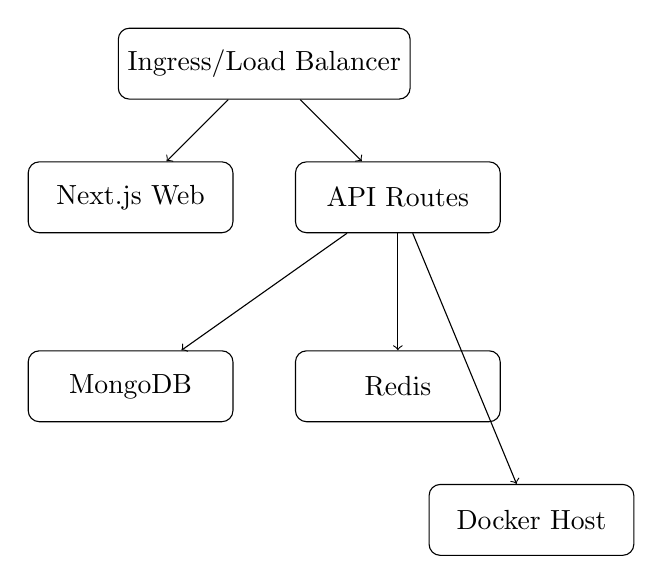
\begin{tikzpicture}[node distance=2.4cm, auto]
  \tikzstyle{svc}=[rectangle, draw, rounded corners, minimum width=2.6cm, minimum height=0.9cm]
  \node[svc] (lb) {Ingress/Load Balancer};
  \node[svc, below left of=lb] (web) {Next.js Web};
  \node[svc, below right of=lb] (api) {API Routes};
  \node[svc, below of=api] (redis) {Redis};
  \node[svc, below of=web] (mongo) {MongoDB};
  \node[svc, below right of=redis] (docker) {Docker Host};
  \draw[->] (lb) -- (web);
  \draw[->] (lb) -- (api);
  \draw[->] (api) -- (redis);
  \draw[->] (api) -- (mongo);
  \draw[->] (api) -- (docker);
\end{tikzpicture}

	\chapter{User Guide}
\section{Getting Started}
\begin{enumerate}
  \item Sign up and log in.
  \item Create a new project and select a template (Node/React/etc.).
  \item Open the editor, explore file tree, and terminal.
\end{enumerate}

\section{Keyboard Shortcuts}
\begin{longtable}{@{}p{5cm} p{9cm}@{}}
\toprule
\textbf{Shortcut} & \textbf{Action} \\
\midrule
\endhead
Ctrl/Cmd + P & Quick open files \\
Ctrl/Cmd + S & Save file \\
Ctrl/Cmd + ` & Toggle terminal \\
Ctrl/Cmd + F & Find in file \\
\bottomrule
\end{longtable}

\section{Troubleshooting}
\begin{itemize}
  \item If a container fails to start, check project logs and retry.
  \item When ports are busy, release or reassign via the Ports panel.
  \item For auth issues, clear cookies and re-authenticate.
\end{itemize}

	\chapter{Packages and Licenses}
This chapter lists the key npm dependencies with their purpose and typical licenses. Verify exact versions and licenses via your lockfile at release time.

\section{Dependencies}
\begin{longtable}{@{}p{4cm} p{8cm} p{2cm}@{}}
\toprule
\textbf{Name} & \textbf{Purpose} & \textbf{License} \\
\midrule
\endhead
next & React framework for SSR/SSG & MIT \\
react & UI components library & MIT \\
react-dom & React DOM renderer & MIT \\
next-auth & Authentication for Next.js & ISC \\
bcryptjs & Password hashing & MIT \\
mongodb & MongoDB Node.js driver & Apache-2.0 \\
ioredis & Redis client & MIT \\
dockerode & Docker remote API client & Apache-2.0 \\
@reduxjs/toolkit & Redux utilities & MIT \\
socket.io & Real-time communication & MIT \\
tailwindcss & Utility-first CSS & MIT \\
shadcn/ui & UI components (radix-based) & MIT \\
\bottomrule
\end{longtable}

\section{Attribution and Citations}
We cite key packages in the bibliography: \cite{nextjs, nextauth, mongodb, redis, dockerode, rtk}. For security standards and practices, see \cite{owasp-asvs, node-best-practices}.

	\chapter{Engineering Best Practices}
\section{Code Quality}
\begin{itemize}
  \item TypeScript everywhere; strict mode enabled.
  \item ESLint and Prettier to enforce conventions.
  \item Small, pure functions and React components; testable services.
\end{itemize}

\section{Security}
\begin{itemize}
  \item Follow OWASP ASVS \cite{owasp-asvs}.
  \item Input validation and output encoding; deny-by-default.
  \item Secrets via environment variables; avoid hardcoding.
\end{itemize}

\section{Performance}
\begin{itemize}
  \item Memoize expensive selectors; code-split routes.
  \item Use streaming where possible for logs and large file reads.
  \item Limit container resources and reuse base images.
\end{itemize}

\section{Reliability}
\begin{itemize}
  \item Retry with backoff for transient errors (DB/Redis/Docker).
  \item Idempotent APIs; structured logs with correlation IDs.
  \item Health checks and readiness probes for services.
\end{itemize}

	\chapter{Results and Discussion}
\section{Overview of Results}

The F1 Simulation Project was designed to provide an engaging and interactive experience of a Formula 1 race. Throughout the simulation, various parameters such as team selection, driver performance, venue characteristics, and weather conditions were evaluated. This section presents the key findings from the simulations conducted.

\subsection{Simulation Outcomes}

The primary outcomes of the simulations can be summarized as follows:

\begin{itemize}
    \item The performance of drivers varied significantly based on their chosen teams and car specifications. Drivers from teams with higher horsepower and better aerodynamics consistently finished in the top positions.
    \item Weather conditions played a crucial role in determining the race outcomes. For instance, rainy weather conditions negatively affected lap times, resulting in a higher number of accidents and slower overall performance.
    \item Different venues introduced unique challenges. The difficulty ratings assigned to each venue influenced the drivers' strategies, with more challenging tracks requiring greater focus and skill.
\end{itemize}

\subsection{Podium Results}

The podium results for each race simulation showcased the top three drivers, highlighting their performance and providing commentary based on their respective teams. This feature not only added excitement to the simulation but also educated users about the significance of teamwork in achieving success in Formula 1 racing.

\subsection{Statistical Analysis}

A detailed statistical analysis of the simulation outcomes revealed the following insights:

\begin{itemize}
    \item \textbf{Average Lap Time:} The average lap time varied across different venues and weather conditions, impacting the overall race duration.
    \item \textbf{Page Fault Rate:} The project implementation also measured the page fault rate in the context of memory management, demonstrating efficient memory usage during simulation execution.
    \item \textbf{Driver Performance Metrics:} Metrics such as average speed, number of laps completed, and incidents during the race were tracked, providing a comprehensive overview of driver performance.
\end{itemize}

\section{Implications of Results}

The results of this simulation not only serve to entertain but also provide valuable insights into the world of Formula 1 racing. The impact of technical specifications on race outcomes emphasizes the importance of engineering in motorsports. Furthermore, the significance of weather conditions and track characteristics illustrates the unpredictable nature of racing.

\subsection{Educational Value}

The F1 Simulation Project has educational implications, particularly for those interested in motorsports, engineering, and programming. It serves as a practical example of how computer simulations can be used to model real-world scenarios and analyze complex systems.

\section{Limitations and Future Work}

While the project has successfully achieved its primary goals, several limitations were identified:

\begin{itemize}
    \item \textbf{Simplified Model:} The simulation uses simplified models for driver performance, which may not capture the full complexity of real-world racing dynamics.
    \item \textbf{Limited Variables:} Future enhancements could include additional variables, such as tire wear and pit stop strategies, to create a more realistic simulation.
\end{itemize}

In future work, it would be beneficial to integrate more sophisticated algorithms and machine learning techniques to predict race outcomes based on historical data. Additionally, expanding the number of teams and drivers could provide a richer simulation experience.

\section{Conclusion}

The F1 Simulation Project successfully provides an engaging and educational platform for exploring the dynamics of Formula 1 racing. The results demonstrate the interplay of various factors in determining race outcomes and emphasize the importance of strategy and teamwork in achieving success on the track.

\end{document}

	\chapter{Conclusion and Future Work}

\section{Conclusion}

The F1 Simulation Project has successfully demonstrated the core principles of Formula 1 racing through a computer simulation. By allowing users to interactively engage with various aspects of the race, the project highlights the importance of several key factors, including driver skill, vehicle specifications, track characteristics, and environmental conditions.

Throughout the project, we developed an engaging platform that simulated race scenarios, tracked driver performance, and provided meaningful commentary on the outcomes. The statistical analysis of the simulation data revealed insights into the dynamics of racing, emphasizing the significance of technical specifications such as horsepower and aerodynamics in determining race outcomes.

The educational value of the project cannot be overstated; it serves as a practical example of how programming and simulation can be leveraged to understand complex systems. The project not only provides entertainment but also fosters a deeper appreciation for the engineering and strategy involved in Formula 1 racing.

\section{Future Work}

While the F1 Simulation Project has met its initial objectives, there are several avenues for future enhancements:

\begin{itemize}
    \item \textbf{Incorporating More Variables:} Future iterations could include additional parameters such as tire wear, pit stop strategies, and driver fatigue to create a more comprehensive simulation of real-world racing.
    \item \textbf{Enhanced AI for Driver Performance:} Integrating machine learning techniques could lead to smarter AI drivers that adapt their strategies based on the simulation environment and player decisions.
    \item \textbf{Real-Time Weather Dynamics:} Implementing a dynamic weather system that affects race conditions in real-time could add an additional layer of complexity and realism to the simulation.
    \item \textbf{Multiplayer Functionality:} Introducing multiplayer features would allow users to compete against one another, simulating real-time races and adding a social element to the experience.
    \item \textbf{Graphical Enhancements:} Improving the graphical interface and visualization of race data could further engage users and enhance the overall experience.
\end{itemize}

\section{Final Thoughts}

In conclusion, the F1 Simulation Project represents a significant achievement in blending programming, simulation, and the excitement of Formula 1 racing. By building upon this foundation, future work can expand the project's scope, offering an even richer and more immersive experience for users.

The lessons learned from this project serve as a stepping stone for further explorations in the field of simulation and modeling. As technology continues to advance, the potential for creating realistic and engaging simulations in motorsports and beyond remains vast and full of possibilities.

\end{document}


	\bibliographystyle{plain}
	\bibliography{report}
 
\end{document}
